\chapter{乡村建设}
\label{chapter:basic}

《乡村建设行动实施方案》指出:乡村建设是实施乡村振兴战略的重要任务,也是国家现代化建设的重要内容。

乡村基础设施的建设不仅是提升乡村生活品质的关键,更是吸引人才和促进人口回流的重要举措。此外乡村地区的文化和自然环境也是其独特的吸引力所在。

\section{基础设施建设}

在具体的基础设施建设中,为了量化评估进展和成效,本文选择了俩个关键性的指标:每万人拥有的卫生床数量和人均养老机构数量。这俩个指标不仅反映了乡村医疗卫生和养老服务设施的发展水平,也是衡量基础设施建设对提升居民生活质量影响的重要参数。

在收集近十年各地区的卫生床和人均养老机构数量数据的过程中\cite{heywhale-dataset},本文采用年复合增长率(CAGR)这一指标,将每个地区过去十年的数据统一转化,以便进行比较。同时进一步制作了一幅详尽的中国热力图,直观展现了各地区在所考察指标上的表现。

\begin{figure}[H]
    \centering
    \begin{minipage}{0.45\textwidth}
        \centering
        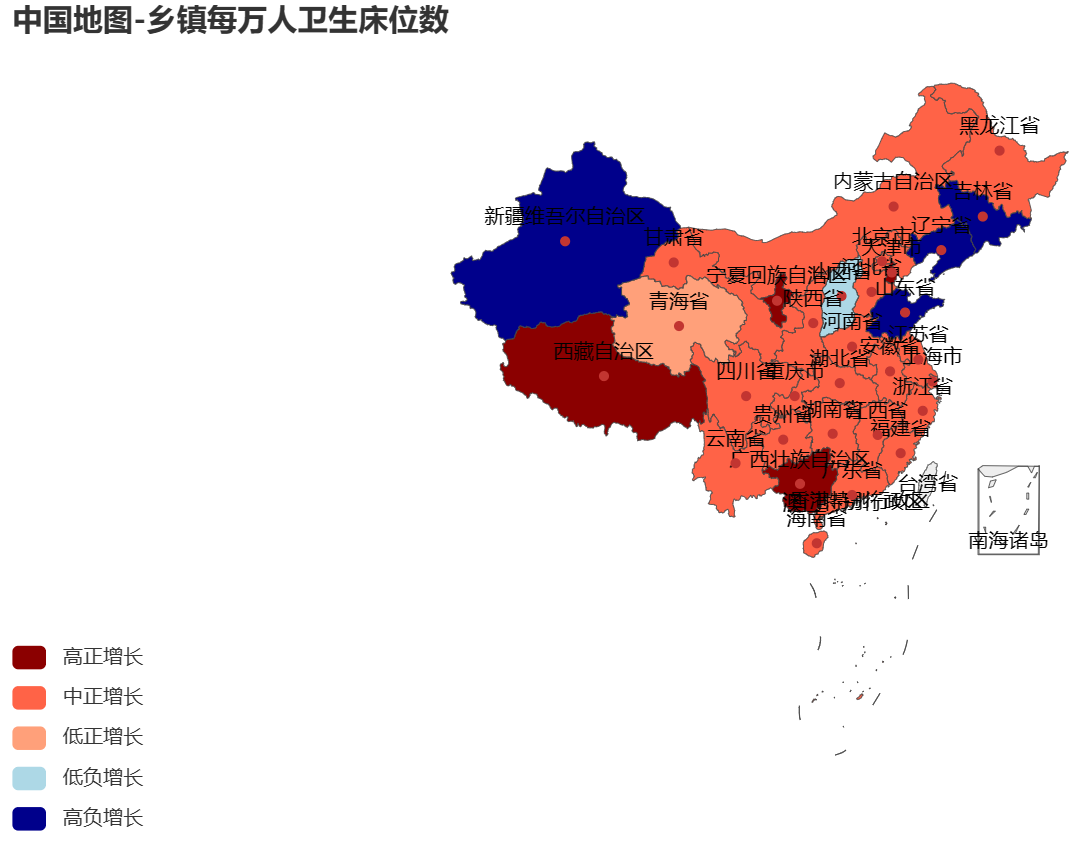
\includegraphics[width=\linewidth]{figures/18.png}
        \caption{卫生床位数}
        \label{fig:beds}
    \end{minipage}\hfill
    \begin{minipage}{0.45\textwidth}
        \centering
        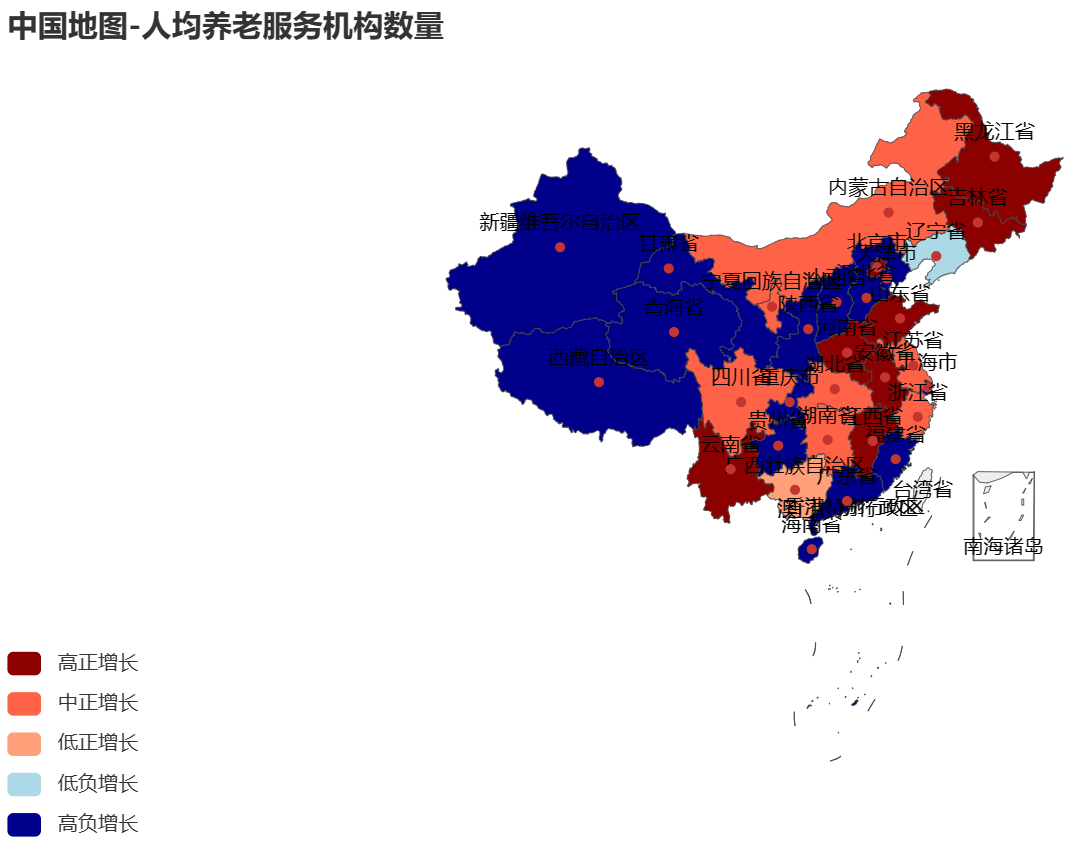
\includegraphics[width=\linewidth]{figures/17.png}
        \caption{养老机构数量}
        \label{fig:elderly-facilities}
    \end{minipage}
\end{figure}

在这两幅图中,红色区域表示正增长区域,蓝色区域表示负增长区域。颜色的深浅代表了增长的强度:红色越深表明正增长程度越高,蓝色越深则意味着负增长程度越显著。

结合胡焕庸线的地理分布来观察,在沿线东部地区,尤其是人口密集的乡镇,无论是卫生床位数还是养老机构数量,普遍呈现出正增长趋势。

然而,胡焕庸线以西的西部地区,尤其是人口较少的农村区域,却出现了卫生床位和养老机构数量的负增长趋势。这种情况在一些经济较发达的地区也有所体现,可能与这些地区的农村人口减少,需求降低有关。

这种差异性的现象揭示了我国农村在基础设施建设方面正处于一个积极变化的发展阶段。东部的积极增长反映了国家对农村地区尤其是人口密集区域的关注和投资的增加,显示出公共服务水平正在逐步提升,以适应居民不断增长的需求。而西部地区则突显了在人口减少的背景下,如何有效地规划和调整基础设施,以持续满足农村居民变化的需求。
\section{基础环境建设}

在推进乡村基础设施建设的过程中,必须同步加强对乡村自然环境的保护和改善,这对于实现乡村振兴和可持续发展具有至关重要的作用。

% "绿水青山就是金山银山"的发展理念深刻阐明了保护和改善自然环境不仅是对生态平衡的维护,更是推动经济和社会进步的关键路径。

本文对乡村环境进行了系统的量化分析,收集并研究了2015至2022年期间的关键环境指标数据\cite{rural-revitalization-environmental-report-2022}。这些数据包括村庄的供水情况、排水管道系统、人均绿地面积、环卫车辆的数量和使用情况以及公共厕所的配置和状况。通过计算连续两年之间的数据差值来确定每年的变化量,绘制出变化量与年份的关系图如下图所示\cite{农质发〔2023〕5号}:

\begin{figure}[H]
    \centering
    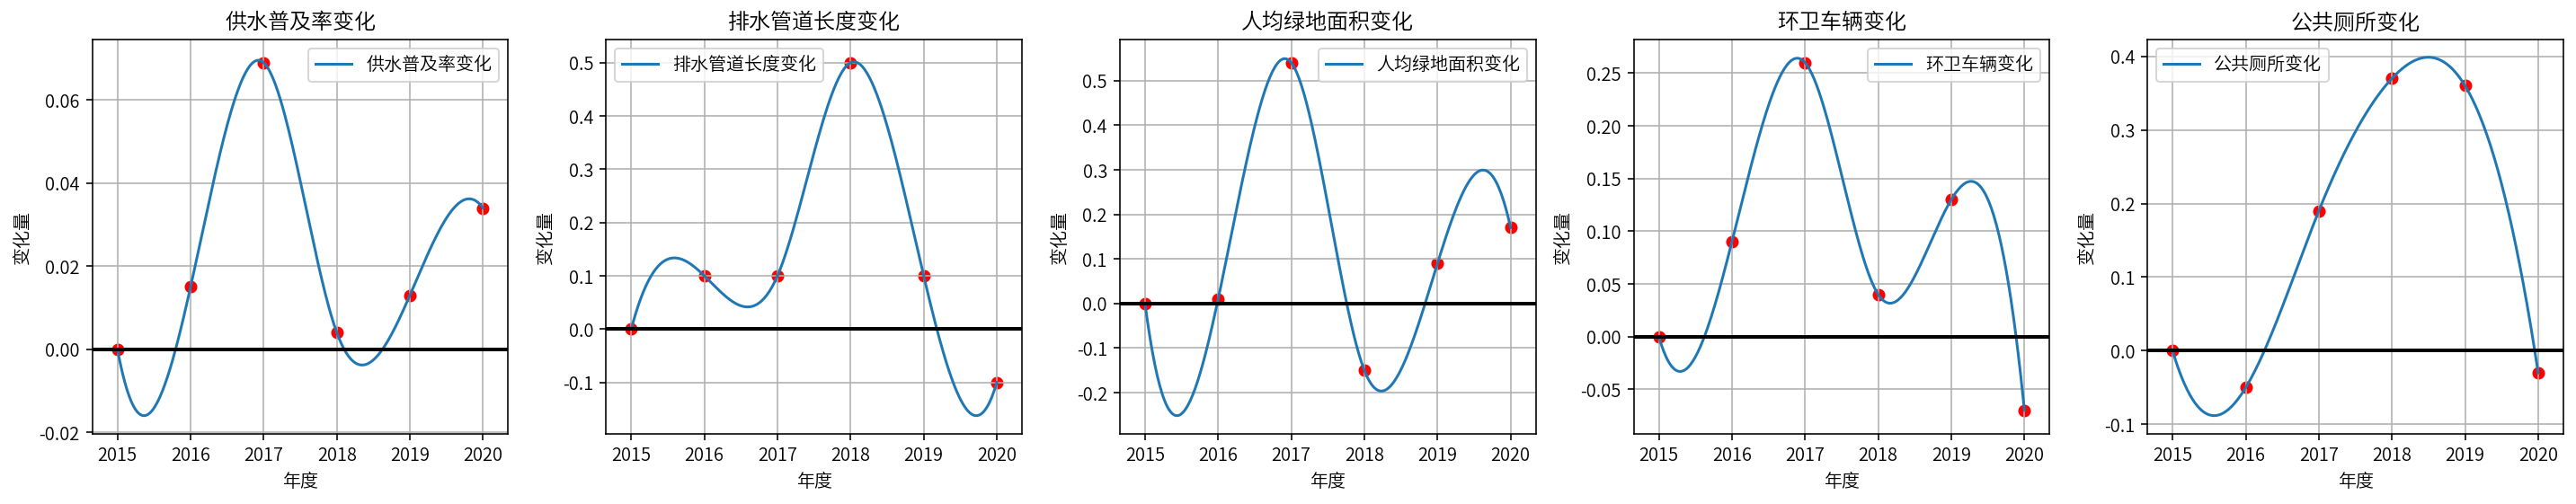
\includegraphics[width=1.0\linewidth]{figures/21.png}
    \caption{基础环境改善图}
    \label{fig:basic_environment}
\end{figure}

图表展示了多个指标随时间变化的趋势,其中大部分曲线持续处于零点线以上。这表明,尽管各指标呈现出明显的波动,总体上还是保持了增长态势。这一现象彰显了国家对基础设施与环境改善的坚定承诺。

\section{生态旅游建设}
乡村环境的改善已成为提升居民生活质量和健康水平的关键因素,同时也开辟了乡村经济转型升级的新路径。

环境质量的提升不仅吸引了生态旅游和绿色农业等绿色经济产业,也促成了新的经济增长点和增加了就业机会,为乡村带来了新的活力。本文深入分析了过去近十年来乡村旅游接待游客数量及其所带来的旅游总收入\cite{bisu-rural-tourism-report},绘制出如下图所示的柱状图:

% 在乡村振兴战略的推动下,乡村旅游特别成为了促进经济多样化、提高农民收入和加强城乡一体化的一个强有力的平台,展现了其在当前和未来乡村发展中的重要作用。

\begin{figure}[h]
    \centering
    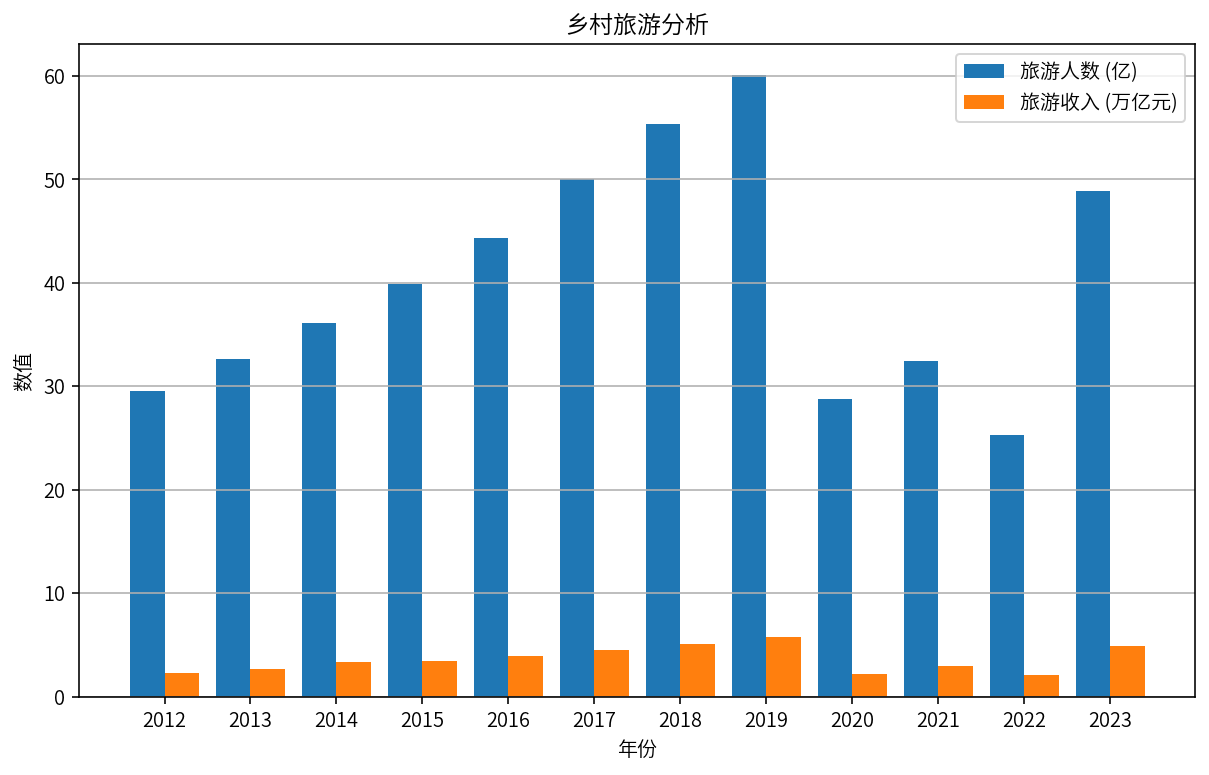
\includegraphics[width=0.65\linewidth]{figures/10.png}
    \caption{近十年乡村旅游人数与旅游收入}
\end{figure}

初期数据显示,乡村旅游人数和收入都呈现出稳步增长的态势,反映了人们对逃离城市喧嚣、探索自然和体验乡村生活愈发浓厚的兴趣。然而,2020年新冠疫情的爆发对我国旅游业造成了前所未有的打击,乡村旅游也未能幸免,其人次和收入均出现了急剧下滑。

随着疫情的结束,乡村旅游业开始呈现出复苏的势头,人们逐渐回归到了疫情前的生活和休闲模式。乡村旅游经历了一段迅猛的增长期,这种增长不仅归功于疫情的消退,乡村基础设施和环境设施的改善也在促进乡村旅游发展中发挥了至关重要的作用。

% 随着疫情逐步得到控制和政府的积极扶持,加之产业结构的优化和转型,乡村旅游开始展现出复苏的迹象。这一趋势不仅反映了乡村旅游的韧性和潜力,也预示着乡村旅游在后疫情时代将持续成为人们休闲和旅游的重要选择。

% 政府政策的支持和对乡村旅游潜力的认识促使相关产业链得到改善和升级,为乡村旅游的恢复提供了强有力的推动。经济逐步复苏,消费者信心增强,人们再次开始探索和享受乡村旅游带来的独特魅力,这促使乡村旅游的人次和收入逐渐恢复并呈现出积极的发展势头。